\documentclass[12pt]{article}
\usepackage{amsmath}
\usepackage{graphicx}
\usepackage{hyperref}
\usepackage{listings}
\usepackage{color}
\usepackage{pythonhighlight}

\title{Operating System Course Report - First Half of the Semester}
\author{B class}
\date{\today}

\begin{document}

\maketitle
\newpage

\tableofcontents
\newpage

\section{Introduction}
This report summarizes the topics covered during the first half of the Operating System course. It includes theoretical concepts, practical implementations, and assignments. The course focuses on the fundamentals of operating systems, including system architecture, process management, CPU scheduling, and deadlock handling.

\section{Course Overview}
\subsection{Objectives}
The main objectives of this course are:
\begin{itemize}
    \item To understand the basic components and architecture of a computer system.
    \item To learn process management, scheduling, and inter-process communication.
    \item To explore file systems, input/output management, and virtualization.
    \item To study the prevention and handling of deadlocks in operating systems.
\end{itemize}

\subsection{Course Structure}
The course is divided into two halves. This report focuses on the first half, which covers:
\begin{itemize}
    \item Basic Concepts and Components of Computer Systems
    \item System Performance and Metrics
    \item System Architecture of Computer Systems
    \item Process Description and Control
    \item Scheduling Algorithms
    \item Process Creation and Termination
    \item Introduction to Threads
    \item File Systems
    \item Input and Output Management
    \item Deadlock Introduction and Prevention
    \item User Interface Management
    \item Virtualization in Operating Systems
\end{itemize}

\section{Topics Covered}

\subsection{Basic Concepts and Components of Computer Systems}
This section explains the fundamental components that make up a computer system, including the CPU, memory, storage, and input/output devices.

\subsection{System Performance and Metrics}
This section introduces various system performance metrics used to measure the efficiency of a computer system, including throughput, response time, and utilization.

\subsection{System Architecture of Computer Systems}
Describes the architecture of modern computer systems, focusing on the interaction between hardware and the operating system.

\subsection{Process Description and Control}
Processes are a central concept in operating systems. This section covers:
\begin{itemize}
    \item Process states and state transitions
    \item Process control block (PCB)
    \item Context switching
\end{itemize}

\subsection{Scheduling Algorithms}
This section covers:
\begin{itemize}
    \item First-Come, First-Served (FCFS)
    \item Shortest Job Next (SJN)
    \item Round Robin (RR)
\end{itemize}
It explains how these algorithms are used to allocate CPU time to processes.

\subsection{Process Creation and Termination}
Details how processes are created and terminated by the operating system, including:
\begin{itemize}
    \item Process spawning
    \item Process termination conditions
\end{itemize}

\subsection{Introduction to Threads}
This section introduces the concept of threads and their relation to processes, covering:
\begin{itemize}
    \item Single-threaded vs. multi-threaded processes
    \item Benefits of multithreading
\end{itemize}

\begin{figure}[h]
    \centering
    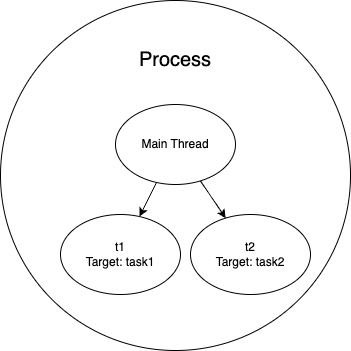
\includegraphics[width=0.5\textwidth]{/Users/khawaritzmi/Unhas/os_report_mid2024/b_class/asset/example.png}  % Sesuaikan nama file dan ukurannya
    \caption{Ini adalah gambar contoh dari multithreading.}
    \label{fig:contoh_gambar}
\end{figure}

Seperti yang terlihat pada Gambar \ref{fig:contoh_gambar}, inilah cara menambahkan gambar dengan keterangan.

\subsection{File Systems}
File adalah unit penyimpanan logika yang diabstraksi oleh sistem operasi dari perangkat penyimpanan. File berisi informasi yang disimpan pada penyimpanan sekunder (seperti \textit{magnetic disk}, \textit{magnetic tape}, dan \textit{optical disk}). Informasi dalam file didefinisikan oleh pembuatnya. Setiap file memiliki struktur tertentu tergantung pada isinya. File dapat terdiri dari data (baik berupa data numerik, karakter, maupun biner) serta program seperti \textit{source program}, \textit{object program}, dan \textit{executable program}.

\subsubsection*{a. Ruang Alamat Logis yang Berdekatan}
File dalam sistem biasanya disimpan sebagai ruang alamat logis yang berdekatan. Hal ini berarti bahwa file menempati urutan alamat logis dalam memori. Namun, hal ini tidak selalu menyiratkan bahwa file juga menempati ruang fisik yang berdekatan pada disk. Sistem file berfungsi untuk menyederhanakan akses dan pengambilan file dengan membuatnya tampak berurutan, terlepas dari bagaimana penyimpanannya secara fisik.

\subsubsection*{b. Jenis File}
File dapat dikategorikan menjadi dua jenis utama:
\begin{enumerate}
    \item \textbf{File Data}: Berisi data terstruktur atau tidak terstruktur dan dapat dikategorikan lebih lanjut menjadi:
    \begin{itemize}
        \item \textbf{Numerik}: Data yang direpresentasikan sebagai angka (misalnya, data statistik atau data keuangan).
        \item \textbf{Character}: Data yang direpresentasikan sebagai teks yang dapat dibaca manusia.
        \item \textbf{Biner}: File non-teks, seperti file media (audio, video), atau jenis data lainnya yang dikodekan.
    \end{itemize}
    \item \textbf{File Program}: File yang berisi kode yang dapat dieksekusi untuk menjalankan aplikasi atau layanan pada komputer.
\end{enumerate}

\subsubsection*{c. Konten File yang Ditentukan oleh Pencipta}
Isi file ditentukan oleh pembuatnya dan tujuan dari pembuatan file tersebut. File yang berbeda mungkin berisi instruksi (\textit{kode sumber}) untuk program komputer, dokumentasi tertulis (file teks), atau kode yang sudah dikompilasi (file \textit{executable}). Contoh jenis file:
\begin{itemize}
    \item \textbf{File Teks}: File sederhana yang berisi karakter yang dapat dibaca oleh manusia.
    \item \textbf{File Sumber}: File yang berisi kode sumber yang ditulis dalam bahasa pemrograman.
    \item \textbf{File yang dapat dieksekusi}: File yang dapat dijalankan langsung oleh sistem operasi sebagai program. File ini berisi kode yang sudah dikompilasi atau ditafsirkan.
\end{itemize}

\subsubsection{File System Structure}
Struktur sistem file mengatur bagaimana file disimpan, diakses, dan diatur dalam perangkat penyimpanan. Struktur ini mencakup beberapa komponen, seperti direktori, tabel alokasi, dan \textit{metadata} yang membantu mengelola file dengan efisien. Struktur file dapat dikategorikan ke dalam berbagai jenis berdasarkan kompleksitas organisasi data. Misalnya:

\begin{enumerate}
    \item \textbf{Simple record Structure}: terdiri dari urutan baris atau catatan dengan panjang tetap atau variabel
    \item \textbf{Complex structures}: lebih rumit mencakup dokumen yang diformat dan file beban yang dapat direlokasi, yang memerlukan mekanisme penanganan yang lebih canggih.
\end{enumerate}

Struktur ini sangat penting dalam mengelola bagaimana data disimpan dan diakses, dan karakter kontrol dapat mensimulasikan struktur yang kompleks. Keputusan tentang organisasi struktur file dipengaruhi oleh sistem operasi dan program yang digunakan. Tipe file juga digunakan untuk menunjukkan struktur internal dari file. File tertentu harus konfirmasi ke struktur yang dibutuhkan yang dimengerti oleh sistem operasi. Misalnya, sistem operasi membutuhkan file \textit{executable} yang mempunyai struktur khusus sehingga dapat menentukan dimana letak memori dan lokasi dari instruksi pertama.

Beberapa sistem operasi menggunakan sekumpulan sistem pendukung struktur file dengan sejumlah operasi khusus untuk manipulasi file dengan struktur tersebut. Hal ini menjadi kelemahan pada sistem operasi yang mendukung struktur file lebih dari satu. Jika sistem operasi menentukan 10 struktur file berbeda, maka perlu menyertakan kode untuk mendukung struktur file tersebut. Setiap file perlu dapat didefinisikan sebagai satu dari tipe file yang didukung oleh sistem operasi. Beberapa sistem operasi seperti UNIX dan MS-DOS hanya mendukung sejumlah struktur file. UNIX menentukan setiap file merupakan deret 8 bit byte dan bit tersebut tidak diterjemahkan oleh sistem operasi. Skema ini mempunyai fleksibilitas maksimum, tetapi sedikit dukungan. Setiap program aplikasi harus menyertakan kode sendiri untuk menterjemahkan file input ke dalam struktur yang tepat. Setidaknya semua SO harus mendukung sedikitnya satu struktur file \textit{executable} sehingga sistem dapat \textit{load} dan menjalankan program.

\subsubsection*{a. File Attributes }
File memiliki nama dan data. Selain itu, ia juga menyimpan informasi meta seperti tanggal dan waktu pembuatan file, ukuran saat ini, tanggal terakhir dimodifikasi, dll. Semua informasi ini disebut atribut sistem file. Berikut adalah beberapa atribut File penting yang digunakan di operasi sistem:

\begin{enumerate}
    \item \textbf Nama: Ini adalah satu-satunya informasi yang disimpan dalam bentuk yang dapat dibaca manusia.
    \item \textbf	Pengidentifikasi: Setiap file diidentifikasi dengan nomor tag unik dalam sistem file yang dikenal sebagai pengidentifikasi.
    \item \textbf Tempat: Menunjuk ke lokasi file di perangkat.	
    \item \textbf Jenis: Atribut ini diperlukan untuk sistem yang mendukung berbagai jenis file.
    \item \textbf Ukuran: Atribut yang digunakan untuk menampilkan ukuran file saat ini.	
    \item \textbf Perlindungan: Atribut ini menetapkan dan mengontrol hak akses membaca, menulis, dan mengeksekusi file.
    \item \textbf Waktu, tanggal, dan keamanan: Ini digunakan untuk perlindungan, keamanan, dan juga digunakan untuk pemantauan
\end{enumerate}

Atribut ini disimpan dalam struktur direktori sistem file, yang memungkinkan sistem operasi untuk mengelola file dengan lebih efisien.

\subsubsection*{b. File Operations}

\begin{enumerate}
    \item \textbf{File sebagai Tipe Data Abstrak}: \\
    File adalah konsep dalam komputasi yang mewakili kumpulan data yang disimpan secara terstruktur. Ini diperlakukan sebagai tipe data abstrak (ADT) karena cara data disimpan dan diakses disembunyikan dari pengguna. Sistem mengabstraksi kompleksitas mengakses dan mengelola data, menyediakan struktur logis bagi pengguna untuk berinteraksi dengan file.
    
    \item \textbf{Buat (Create)}: \\
    Pembuatan file dalam sistem file melibatkan alokasi ruang dan menginisialisasi metadata file. Metadata mencakup nama file, jenis, ukuran, dan atribut lain yang diperlukan agar file dikelola dalam sistem. File yang baru dibuat mungkin kosong pada awalnya dan siap untuk ditulis.
    
    \item \textbf{Tulis (Write)}: \\
    Menulis ke file berarti memasukkan data ke dalam file, dimulai dari lokasi penunjuk tulis saat ini. Proses ini menambahkan data baru atau mengganti data yang ada pada posisi yang ditentukan dalam file. Jika file tidak ada, beberapa sistem akan membuat file baru untuk menyimpan data.
    
    \item \textbf{Baca (Read)}: \\
    Operasi baca mengambil data dari file mulai dari lokasi penunjuk baca saat ini. Penunjuk menunjukkan di mana dalam file sistem harus mulai membaca. Setelah data dibaca, data dimuat ke dalam memori untuk digunakan atau diproses lebih lanjut oleh program.
    
    \item \textbf{Reposisi dalam File -- Cari}: \\
    Operasi pencarian mengubah posisi penunjuk baca atau tulis dalam file tanpa membaca atau menulis data apa pun. Ini memungkinkan sistem untuk menavigasi ke berbagai bagian file dengan cepat. Misalnya, pindah ke akhir file untuk menambahkan data atau pergi ke lokasi tertentu untuk mengubah informasi yang ada.
    
    \item \textbf{Hapus (Delete)}: \\
    Operasi hapus menghapus file dari sistem file. Itu dapat menghapus seluruh file atau menandai ruang yang ditempatinya sebagai tersedia untuk data baru, tergantung pada sistem file yang digunakan. Dalam kebanyakan kasus, metadata dan referensi ke file juga dihapus.
    
    \item \textbf{Truncate}: \\
    Pemotongan mengurangi ukuran file dengan memotong kontennya dari titik tertentu dan seterusnya. Operasi ini berguna ketika ukuran file perlu dikurangi, sambil tetap menjaga file itu sendiri dan metadatanya tetap utuh.
    
    \item \textbf{Open (Buka)}: \\
    Saat file dibuka, sistem mengambil metadatanya dari struktur direktori dan memuatnya ke dalam memori. Deskriptor file dibuat, memungkinkan operasi berikutnya (seperti membaca atau menulis) dilakukan. Membuka file juga mengatur penunjuk baca/tulis ke posisi yang sesuai.
    
    \item \textbf{Close (Tutup)}: \\
    Menutup file berarti menyelesaikan operasi yang tersisa (seperti membilas data yang di-buffer ke disk) dan menghapus informasi file dari memori. Operasi ini memastikan bahwa tidak ada operasi lebih lanjut yang dapat dilakukan pada file hingga file tersebut dibuka kembali.
\end{enumerate}
\subsubsection*{c. Open Files}



Manajemen \textit{open files} adalah salah satu elemen penting dalam sistem operasi modern, karena pada dasarnya, setiap proses yang berjalan sering kali berinteraksi dengan file untuk membaca data, menulis informasi, atau mengakses sumber daya tertentu. Oleh karena itu, manajemen \textit{open files} yang efektif akan berdampak langsung pada kinerja. Beberapa komponen utama yang dibutuhkan untuk mengelola file:

\begin{enumerate}
    \item \textbf{Tabel file terbuka}: \\
    Struktur ini melacak semua file yang sedang dibuka oleh proses. Setiap entri biasanya berisi informasi tentang file, seperti penunjuk file, deskriptor file, dan detail relevan lainnya. Tabel file terbuka sangat penting untuk manajemen file yang efisien dalam sistem operasi. Tanpa tabel ini, sistem operasi akan kesulitan melacak file mana yang terbuka dan oleh proses mana. Tabel ini menyediakan kontrol terpusat untuk penanganan file.

    \item \textbf{Penunjuk berkas}: \\
    Ini merujuk pada penunjuk yang menyimpan posisi baca/tulis terakhir dalam berkas. Penunjuk ini biasanya disimpan per proses untuk melacak posisi tertentu tempat operasi akan dilanjutkan. Penunjuk berkas memungkinkan setiap proses mempertahankan posisinya di dalam berkas secara independen. Hal ini penting dalam lingkungan multitugas di mana beberapa proses dapat membaca atau menulis ke berkas yang sama.

    \item \textbf{Jumlah file yang dibuka}: \\
    Penghitung digunakan untuk melacak berapa banyak proses yang telah membuka berkas tertentu. Hal ini berguna untuk memastikan bahwa entri berkas dalam tabel berkas yang dibuka hanya dihapus setelah proses terakhir menutup berkas tersebut. Penghitung berkas yang dibuka membantu memastikan bahwa berkas tidak dihapus sebelum waktunya dari tabel berkas yang masih digunakan oleh proses lain. Mekanisme ini menyediakan cara penghitungan referensi yang sederhana namun efektif.

    \item \textbf{Lokasi disk berkas}: \\
    \textit{Cache} yang menyimpan informasi mengenai lokasi fisik berkas pada disk, yang memungkinkan akses lebih cepat selama operasi. \textit{Caching} lokasi disk mengurangi operasi I/O disk dengan melacak data akses file dalam memori, sehingga menghasilkan kecepatan akses yang lebih cepat.

    \item \textbf{Hak akses}: \\
    Izin yang dimiliki setiap proses terkait berkas tertentu. Misalnya, suatu proses mungkin memiliki hak baca, tulis, atau eksekusi berdasarkan mode aksesnya. Hak akses menegakkan keamanan dan memastikan bahwa proses hanya dapat berinteraksi dengan berkas sesuai dengan cara yang diizinkan, mencegah akses atau modifikasi yang tidak sah.

\end{enumerate}


\subsubsection*{d. Tipe File}

\begin{table}[htbp] % Optional: For floating position
    \centering
    \begin{tabular}{|c|c|p{6cm}|p{8cm}|} % Defines number of columns and alignment (c = center, l = left, r = right). '|' creates vertical lines.
    \hline
\textbf{Tipe File}      & \textbf{Ekstensi biasa}        & \textbf{Fungsi}                                                      \\ \hline
\textit{Execute}              & exe, com, bin or none           & Baca untuk menjalankan program bahasa mesin                                   \\ \hline
Objek                  & obj, o                          & Dikompilasi, bahasa mesin tidak ditautkan                                  \\ \hline
\textit{Source code}             & c, cc, java, pas, asm, a        & Kode sumber dalam berbagai bahasa                                      \\ \hline
\textit{Batch}                   & bat, sh                        & Perintah ke penerjemah perintah                                    \\ \hline
Teks                   & txt, doc                        & Data tekstual, dokumen                                                 \\ \hline
Pengolah          & wp, tex, rrf, doc            & Berbagai format pengolah kata                                          \\ \hline
\textit{Library}                & lib, a, so                & Berisi pustaka rutinitas untuk pemrograman                                   \\ \hline
Cetak atau Lihat           & arc, zip, tar                  & Format untuk mencetak atau melihat file ASCII atau biner.              \\ \hline
Arsip                 & {arc, zip, tar                   & File-file terkait dikelompokkan menjadi satu file terkompresi untuk arsip atau penyimpanan. \\ \hline
\textit{Multimedia}              & mpeg, mov, rm                  & Berisi informasi audio/video                       \\ \hline
\end{tabular}

    \caption{Tipe File}
    \label{tab:your_label}
\end{table}

Salah satu pertimbangan penting dalam merancang sistem file dan keseluruhan sistem operasi adalah apakah sistem operasi mengenali dan mendukung sistem file. Bila sistem operasi mengenali tipe suatu file, maka dapat dilakukan operasi terhadap file dengan lebih baik.

UNIX menggunakan \textit{magic number} yang disimpan pada awal file untuk mengindikasikan tipe file berupa program \textit{executable}, \textit{batch file} (shell script), file \textit{postscript}, dan lain-lain. Tidak semua file mempunyai \textit{magic number}, sehingga informasi tipe tidak dapat digambarkan. UNIX tidak menyimpan nama dari program pembuatnya. UNIX juga mengizinkan nama ekstensi dari file tersembunyi, sehingga pengguna dapat menentukan tipe file sendiri dan tidak tergantung pada sistem operasi.

\subsubsection File access methods
\subsubsection Directory management

\end{itemize}

\subsection{Input and Output Management}
Input and output management is key for handling the interaction between the system and external devices. This section includes:
\begin{itemize}
    \item Device drivers
    \item I/O scheduling
\end{itemize}

\subsection{Deadlock Introduction and Prevention}
Explores the concept of deadlocks and methods for preventing them:
\begin{itemize}
    \item Deadlock conditions
    \item Deadlock prevention techniques
\end{itemize}

\subsection{User Interface Management}
This section discusses the role of the operating system in managing the user interface. Topics covered include:
\begin{itemize}
    \item Graphical User Interface (GUI)
    \item Command-Line Interface (CLI)
    \item Interaction between the user and the operating system
\end{itemize}

\subsection{Virtualization in Operating Systems}
Virtualization allows multiple operating systems to run concurrently on a single physical machine. This section explores:
\begin{itemize}
    \item Concept of virtualization
    \item Hypervisors and their types
    \item Benefits of virtualization in modern computing
\end{itemize}

\section{Assignments and Practical Work}
\subsection{Assignment 1: Process Scheduling}
Students were tasked with implementing various process scheduling algorithms (e.g., FCFS, SJN, and RR) and comparing their performance under different conditions.
\subsubsection{Group 1}
\begin{python}
    class Process:
    def __init__(self, pid, arrival_time, burst_time):
        self.pid = pid
        self.arrival_time = arrival_time
        self.burst_time = burst_time
        self.completion_time = 0
        self.turnaround_time = 0
        self.waiting_time = 0
\end{python}

\begin{table}[htbp] % Optional: For floating position
    \centering
    \begin{tabular}{|c|c|c|} % Defines number of columns and alignment (c = center, l = left, r = right). '|' creates vertical lines.
    \hline
    Header 1 & Header 2 & Header 3 \\ % Column headers
    \hline
    Row 1, Column 1 & Row 1, Column 2 & Row 1, Column 3 \\ % First row of data
    \hline
    Row 2, Column 1 & Row 2, Column 2 & Row 2, Column 3 \\ % Second row of data
    \hline
    \end{tabular}
    \caption{Your table caption} % Optional: For adding a caption
    \label{tab:your_label} % Optional: For cross-referencing the table
\end{table}

\subsubsection{}
\subsubsection{}
\subsubsection{}
\subsubsection{}
\subsubsection{}
\subsubsection{}
\subsubsection{Group 8}
Implementasikan algoritma penjadwalan proses \textit{First Come First Serve} (FCFS). Ada 4 proses dengan \textit{arrival time} dan \textit{burst time} sebagai berikut:
\begin{itemize}
    \item P1: Arrival Time = 0, Burst Time = 5
    \item P2: Arrival Time = 1, Burst Time = 3
    \item P3: Arrival Time = 2, Burst Time = 8
    \item P4: Arrival Time = 3, Burst Time = 6
\end{itemize}
Hitung \textit{waiting time} dan \textit{turnaround time} untuk setiap proses.
\begin{table}[htbp] % Optional: For floating position
    \centering
    \begin{tabular}{|c|c|c|} % Defines number of columns and alignment (c = center, l = left, r = right). '|' creates vertical lines.
    \hline
    Proses  & Arrival Time  & Burst Time  \\ % Column headers
    \hline
    1  & 0 & 5 \\ % First row of data
    \hline
    2 & 1 &3 \\
    \hline
    3 & 2 & 8 \\
    \hline
    4 & 3 & 6 \\
    
    \hline
    \end{tabular}
    \caption{Tabel Data Proses} % Optional: For adding a caption
    \label{tab:your_label} % Optional: For cross-referencing the table
\end{table}

\begin{python}
    
# FCFS Scheduling
def fcfs_scheduling(processes, burst_time, arrival_time):
    n = len(processes)
    waiting_time = [0] * n
    turnaround_time = [0] * n
    
    # Service time calculation
    service_time = [0] * n
    service_time[0] = arrival_time[0]
    
    for i in range(1, n):
        service_time[i] = service_time[i - 1] + burst_time[i - 1]
        waiting_time[i] = service_time[i] - arrival_time[i]
        waiting_time[i] = max(waiting_time[i], 0)

    # Turnaround time calculation
    for i in range(n):
        turnaround_time[i] = burst_time[i] + waiting_time[i]

    avg_waiting_time = sum(waiting_time) / n
    avg_turnaround_time = sum(turnaround_time) / n

    return waiting_time, turnaround_time, avg_waiting_time, avg_turnaround_time

# SJN Scheduling (non-preemptive)
def sjn_scheduling(processes, burst_time, arrival_time):
    n = len(processes)
    waiting_time = [0] * n
    turnaround_time = [0] * n
    completed = [False] * n
    time = 0
    completed_count = 0
    
    while completed_count < n:
        min_bt = float('inf')
        min_index = -1
        
        for i in range(n):
            if arrival_time[i] <= time and not completed[i] and burst_time[i] < min_bt:
                min_bt = burst_time[i]
                min_index = i
        
        if min_index == -1:
            time += 1
            continue
        
        waiting_time[min_index] = time - arrival_time[min_index]
        time += burst_time[min_index]
        turnaround_time[min_index] = time - arrival_time[min_index]
        completed[min_index] = True
        completed_count += 1

    avg_waiting_time = sum(waiting_time) / n
    avg_turnaround_time = sum(turnaround_time) / n

    return waiting_time, turnaround_time, avg_waiting_time, avg_turnaround_time

# Round Robin Scheduling
def rr_scheduling(processes, burst_time, arrival_time, time_quantum):
    n = len(processes)
    waiting_time = [0] * n
    turnaround_time = [0] * n
    remaining_bt = burst_time[:]
    time = 0
    complete = 0
    
    while complete < n:
        for i in range(n):
            if remaining_bt[i] > 0:
                if remaining_bt[i] > time_quantum:
                    time += time_quantum
                    remaining_bt[i] -= time_quantum
                else:
                    time += remaining_bt[i]
                    waiting_time[i] = time - burst_time[i] - arrival_time[i]
                    turnaround_time[i] = time - arrival_time[i]
                    remaining_bt[i] = 0
                    complete += 1

    avg_waiting_time = sum(waiting_time) / n
    avg_turnaround_time = sum(turnaround_time) / n

    return waiting_time, turnaround_time, avg_waiting_time, avg_turnaround_time

# Fungsi untuk membandingkan algoritma
def compare_algorithms(processes, burst_time, arrival_time, time_quantum):
    print("== FCFS ==")
    wt_fcfs, tat_fcfs, avg_wt_fcfs, avg_tat_fcfs = fcfs_scheduling(processes, burst_time, arrival_time)
    print(f"Average Waiting Time: {avg_wt_fcfs:.2f}")
    print(f"Average Turnaround Time: {avg_tat_fcfs:.2f}\n")

    print("== SJN ==")
    wt_sjn, tat_sjn, avg_wt_sjn, avg_tat_sjn = sjn_scheduling(processes, burst_time, arrival_time)
    print(f"Average Waiting Time: {avg_wt_sjn:.2f}")
    print(f"Average Turnaround Time: {avg_tat_sjn:.2f}\n")

    print("== Round Robin ==")
    wt_rr, tat_rr, avg_wt_rr, avg_tat_rr = rr_scheduling(processes, burst_time, arrival_time, time_quantum)
    print(f"Average Waiting Time: {avg_wt_rr:.2f}")
    print(f"Average Turnaround Time: {avg_tat_rr:.2f}\n")

# Data proses
processes = ['P1', 'P2', 'P3', 'P4']
burst_time = [5, 3, 8, 6]
arrival_time = [0, 1, 2, 3]
time_quantum = 2

compare_algorithms(processes, burst_time, arrival_time, time_quantum)

\end{python}


\subsection{Assignment 2: Deadlock Handling}
In this assignment, students were asked to simulate different deadlock scenarios and explore various prevention methods.

\subsection{Assignment 3: Multithreading and Amdahl's Law}
This assignment involved designing a multithreading scenario to solve a computationally intensive problem. Students then applied **Amdahl's Law** to calculate the theoretical speedup of the program as the number of threads increased.
\subsubsection{}
\subsubsection{}
\subsubsection{}
\subsubsection{}
\subsubsection{}
\subsubsection{}
\subsubsection{Group 8}
Buat sebuah skenario \textit{multithreading}  untuk menyelesaikan masalah komputasi \textit{intensif}, seperti menghitung elemen terbesar dalam sebuah \textit{array} besar. Implementasikan kode Python untuk menghitung elemen terbesar menggunakan \textit{multithreading} dan hitung \textit{speedup teoritis} menggunakan \textit{Amdahl's Law} saat jumlah \textit{thread} meningkat.
\begin{python}
    import threading
    import random
    import time
    
    
    def find_max(arr, result, index):
        result[index] = max(arr)
    
    
    def amdahls_law(serial_fraction, n_threads):
        parallel_fraction = 1 - serial_fraction
        speedup = 1 / (serial_fraction + (parallel_fraction / n_threads))
        return speedup
    
    
    def multithreaded_max(arr, num_threads):
        chunk_size = len(arr) // num_threads
        threads = []
        results = [0] * num_threads
    
        for i in range(num_threads):
            chunk = arr[i*chunk_size : (i+1)*chunk_size] if i != num_threads - 1 else arr[i*chunk_size:]
            t = threading.Thread(target=find_max, args=(chunk, results, i))
            threads.append(t)
            t.start()
    
        for t in threads:
            t.join()
    
        overall_max = max(results)
        return overall_max
    
    
    arr_size = 1000000
    arr = [random.randint(1, 1000000) for _ in range(arr_size)]
    
    
    n_threads_list = [1, 2, 4, 8]
    serial_fraction = 0.1  # Assuming 10% of the code is not parallelizable
    
    print("Finding the maximum element in the array...")
    for n_threads in n_threads_list:
        start_time = time.time()
        max_element = multithreaded_max(arr, n_threads)
        end_time = time.time()
    
        elapsed_time = end_time - start_time
        print(f"Number of threads: {n_threads}, Maximum element: {max_element}, Time taken: {elapsed_time:.4f} seconds")
    
        
        theoretical_speedup = amdahls_law(serial_fraction, n_threads)
        print(f"Theoretical Speedup with {n_threads} threads: {theoretical_speedup:.2f}\n")    
\end{python}

\subsection{Assignment 4: Simple Command-Line Interface (CLI) for User Interface Management}
Students were tasked with creating a simple **CLI** for user interface management. The CLI should support basic commands such as file manipulation (creating, listing, and deleting files), process management, and system status reporting.

\subsection{Assignment 5: File System Access}
In this assignment, students implemented file system access routines, including:
\begin{itemize}
    \item File creation and deletion
    \item Reading from and writing to files
    \item Navigating directories and managing file permissions
\end{itemize}

\section{Conclusion}
The first half of the course introduced core operating system concepts, including process management, scheduling, multithreading, and file system access. These topics provided a foundation for more advanced topics to be covered in the second half of the course.

\end{document}